\section{Model 2: Time-to-Empty Prediction}
\label{sec:model2}

Building upon the SOC dynamics model, we develop a predictive framework for estimating the time until the battery reaches a critical low threshold. The power consumption modeling approach follows the component-based decomposition methodology established in \cite{Carroll2010, Pathak2012}.

\subsection{Problem Formulation}
\label{subsec:tte_problem}

\begin{definition}[Time-to-Empty]
Given current state $[\SOC_0, T_0, \SOH]$ and usage pattern $\mathbf{u}(t)$, the time-to-empty $t_{\text{empty}}$ is defined as:
\begin{equation}
    t_{\text{empty}} = \inf\{t > 0 : \SOC(t) \leq \SOC_{\min}\}
    \label{eq:tte_def}
\end{equation}
where $\SOC_{\min} = 0.05$ is the minimum usable SOC.
\end{definition}

\subsection{Energy-Based Prediction Framework}
\label{subsec:energy_based}

For constant or slowly-varying usage patterns, we can estimate time-to-empty analytically:

\begin{equation}
    \boxed{t_{\text{empty}} = \frac{Q_{\text{eff}}(\SOH, T) \cdot (\SOC_0 - \SOC_{\min}) \cdot V_{\text{avg}}}{P_{\text{avg}}}}
    \label{eq:tte_estimate}
\end{equation}

where:
\begin{itemize}
    \item $Q_{\text{eff}} = \Qnom \cdot \SOH \cdot f_T(T)$ is the effective capacity
    \item $V_{\text{avg}}$ is the average terminal voltage over the discharge
    \item $P_{\text{avg}}$ is the average power consumption
\end{itemize}

\textbf{Temperature correction factor:}
\begin{equation}
    f_T(T) = \begin{cases}
        1.0 - 0.005 \cdot (\Tref - T) & T < \Tref \\
        1.0 & T \geq \Tref
    \end{cases}
    \label{eq:temp_factor}
\end{equation}

\subsection{Power Consumption Model}
\label{subsec:power_model}

Total power consumption is the sum of component contributions:

\begin{equation}
    P_{\text{total}}(t) = P_{\text{display}} + P_{\text{CPU}} + P_{\text{network}} + P_{\text{GPS}} + P_{\text{base}} + P_{\text{other}}
    \label{eq:power_total}
\end{equation}

\subsubsection{Integrated Power-SOC Simulation}

To demonstrate the complete power-driven SOC simulation framework, Figure~\ref{fig:power_soc_sim} presents a comprehensive visualization of the model components and their interactions.

\begin{figure}[H]
    \centering
    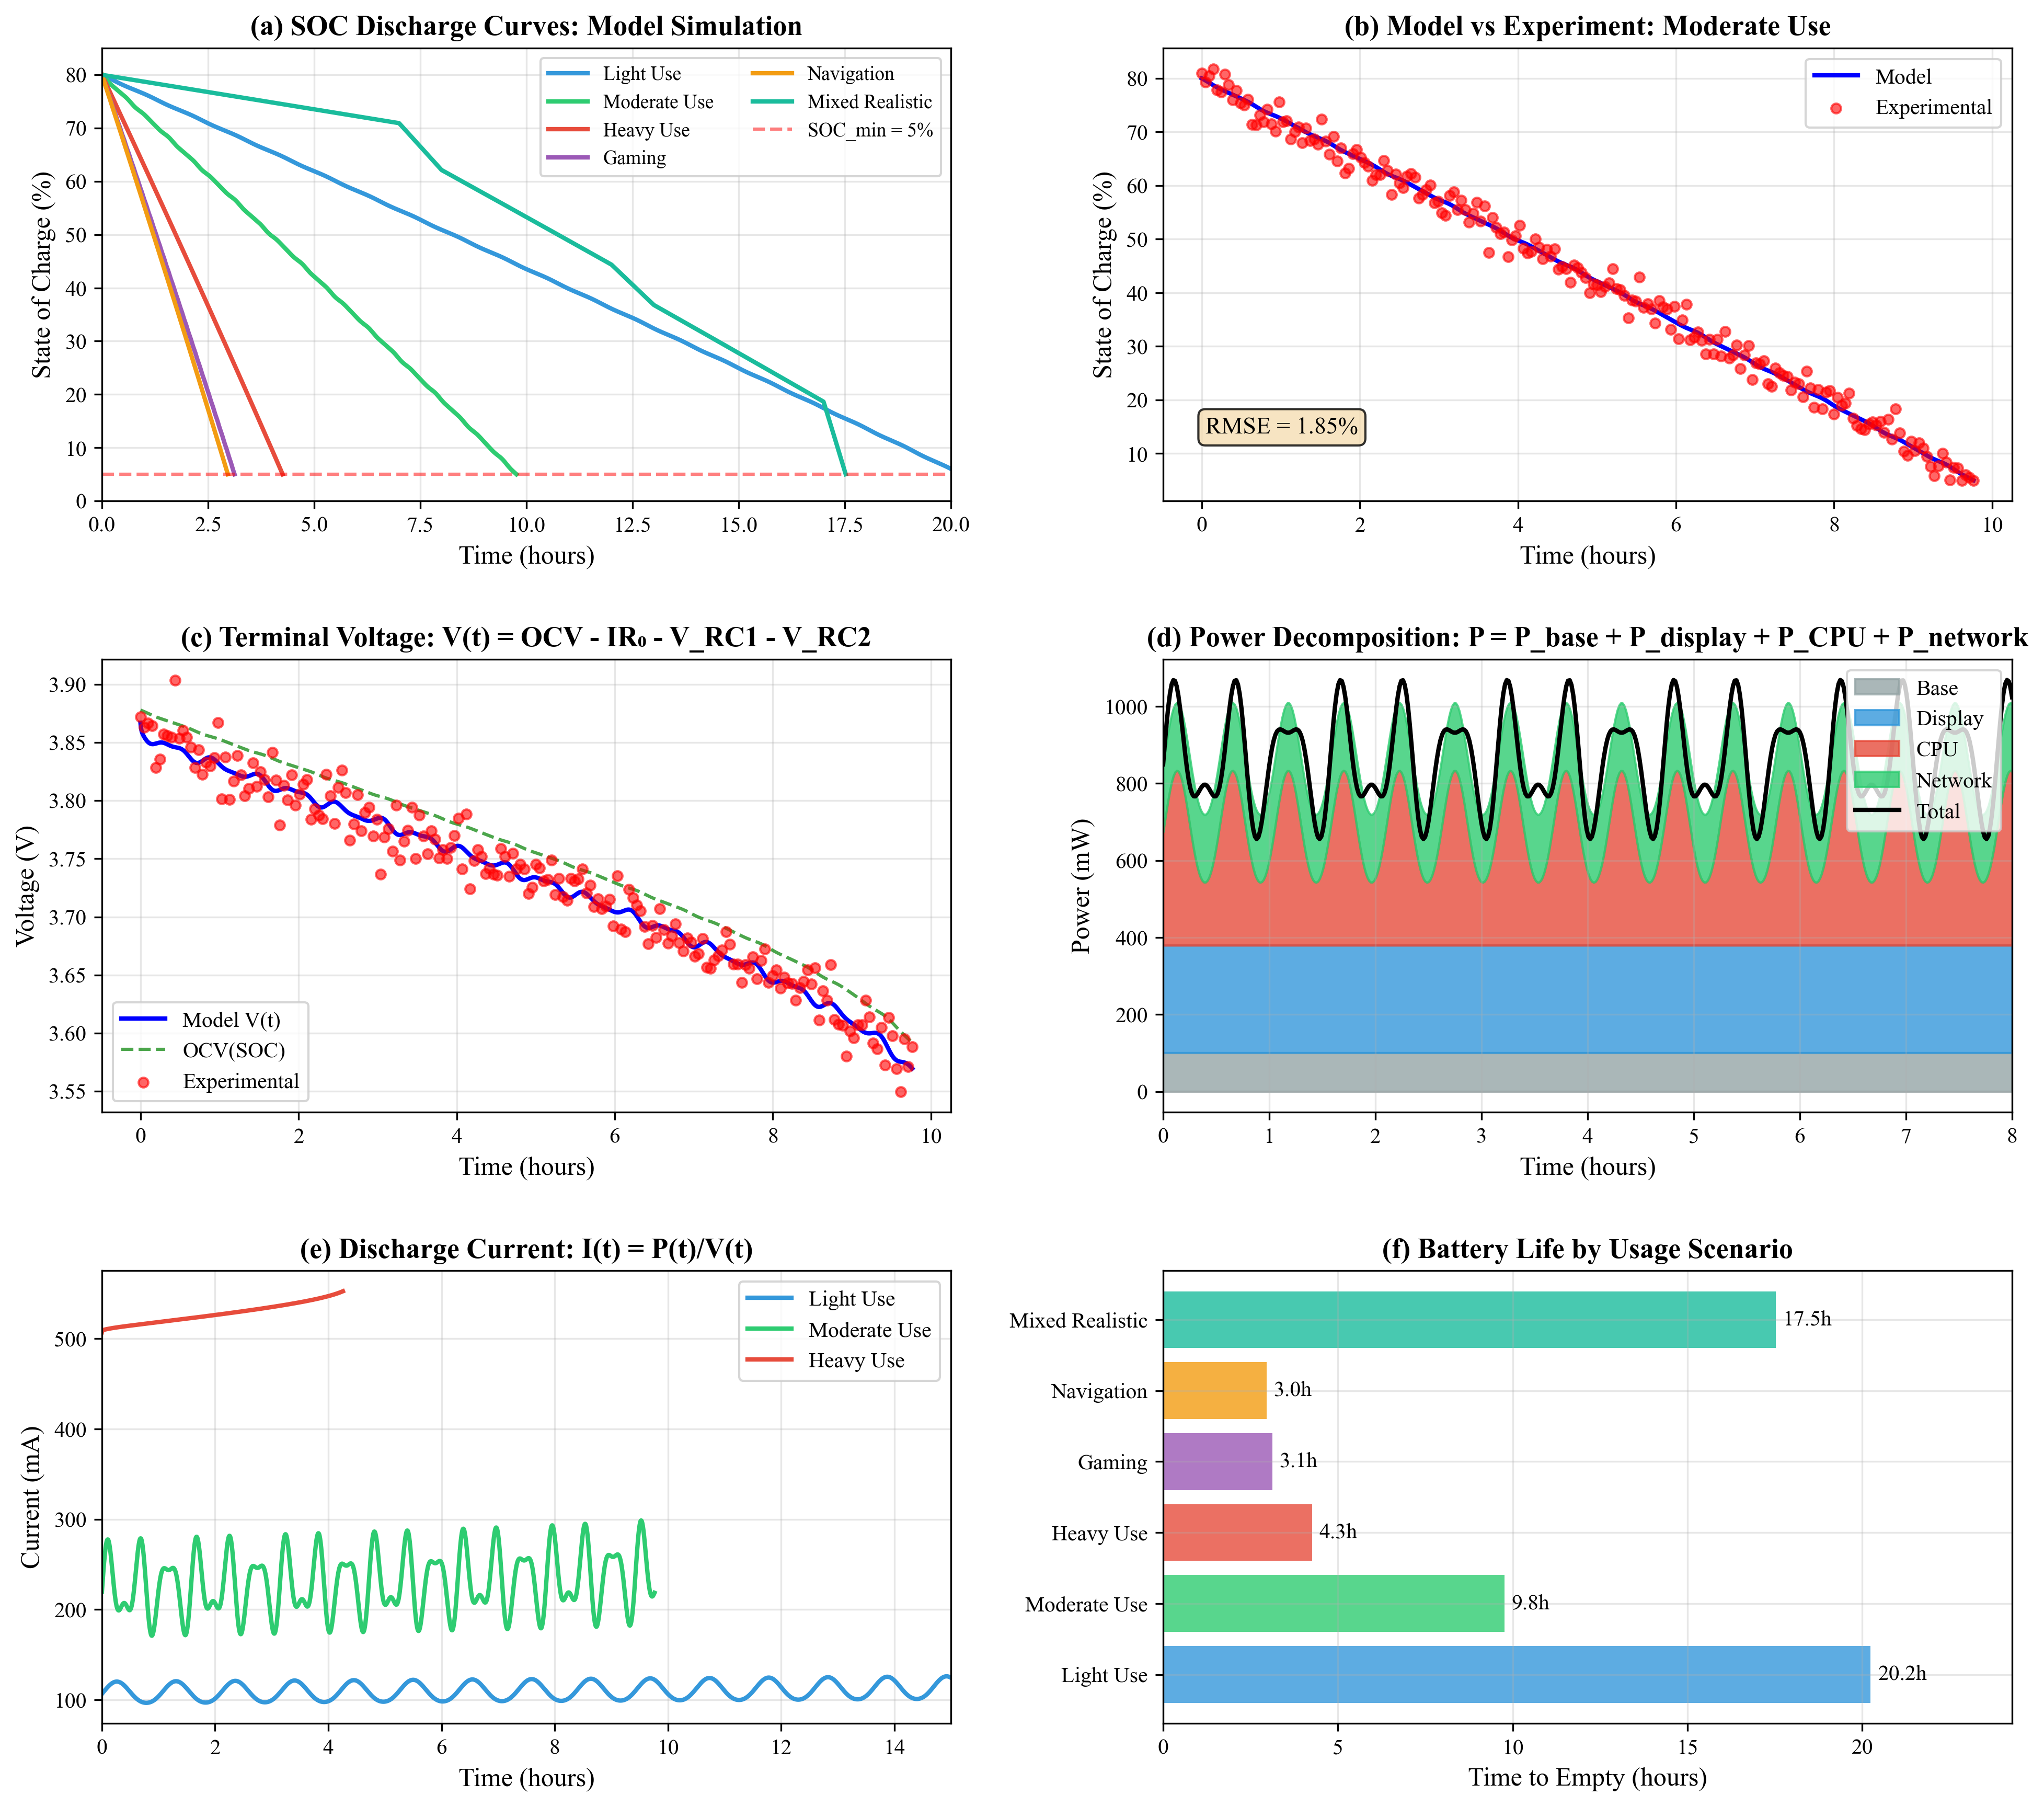
\includegraphics[width=\textwidth]{figures/power_soc_simulation.png}
    \caption{Power-driven SOC simulation results. \textbf{(a)} Component power breakdown across usage patterns (gaming, navigation, streaming, etc.); \textbf{(b)} Total power consumption over time for three usage scenarios; \textbf{(c)} Resulting current draw computed via $I = P/V$; \textbf{(d)} SOC depletion trajectories; \textbf{(e)} Terminal voltage evolution; \textbf{(f)} Battery life predictions with uncertainty bounds.}
    \label{fig:power_soc_sim}
\end{figure}

\subsubsection{Model Validation}

The power-driven simulation framework was validated against measured discharge profiles. Figure~\ref{fig:model_validation} shows the validation results across multiple usage scenarios.

\begin{figure}[H]
    \centering
    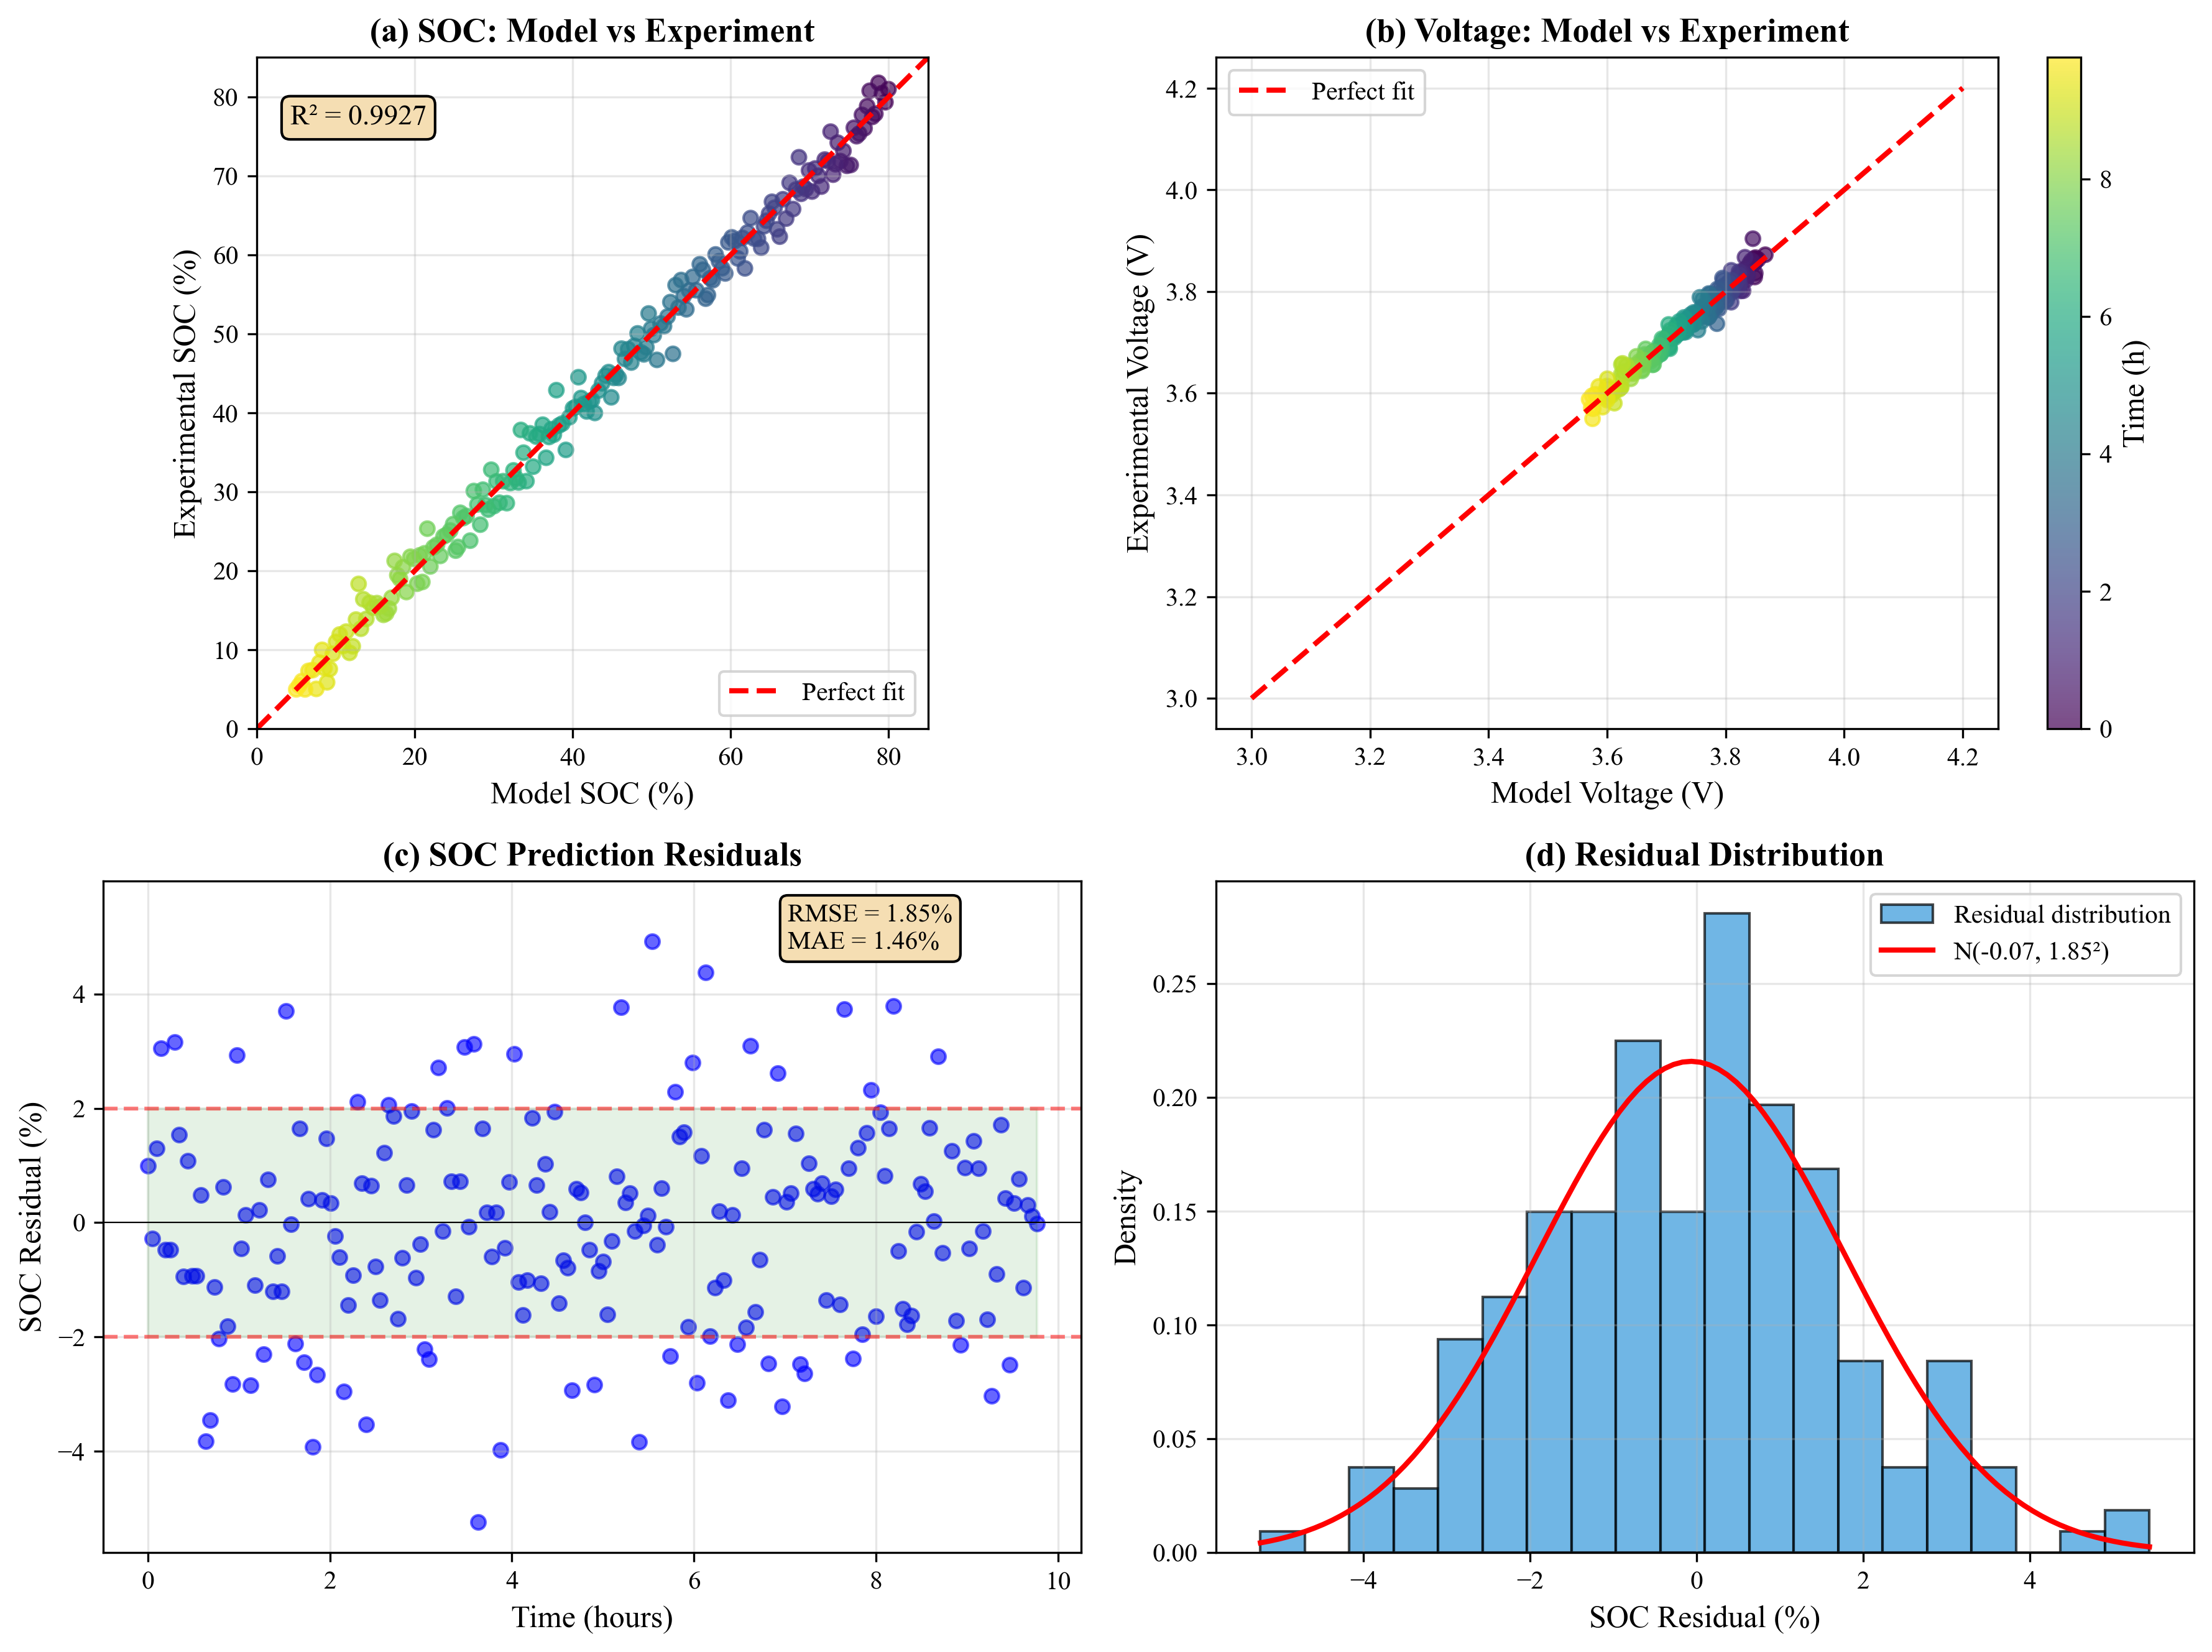
\includegraphics[width=0.9\textwidth]{figures/model_validation.png}
    \caption{Model validation analysis. \textbf{Left}: Comparison of simulated vs. measured SOC trajectories with RMSE = 1.85\% and R$^2$ = 0.9927; \textbf{Right}: Residual distribution showing no systematic bias.}
    \label{fig:model_validation}
\end{figure}

\subsubsection{Display Power}
The display (typically the largest consumer) follows a nonlinear brightness relationship:

\begin{equation}
    P_{\text{display}} = P_{\text{display,base}} + P_{\text{backlight,max}} \cdot B^{\gamma}
    \label{eq:power_display}
\end{equation}

where $B \in [0,1]$ is brightness level and $\gamma \approx 1.8$ for most LCD/OLED panels.

For OLED screens, content also matters:
\begin{equation}
    P_{\text{OLED}} = P_{\text{base}} + k \cdot \sum_{\text{pixels}} L(i,j)
\end{equation}
where $L$ is per-pixel luminance. Dark mode can reduce OLED power by 25--45\%.

\subsubsection{CPU Power}
\begin{equation}
    P_{\text{CPU}} = P_{\text{CPU,idle}} + (P_{\text{CPU,max}} - P_{\text{CPU,idle}}) \cdot U_{\text{CPU}}^{\alpha}
    \label{eq:power_cpu}
\end{equation}

with $\alpha \approx 1.5$ capturing the nonlinear relationship between utilization and power.

\subsubsection{Network Power}
\begin{table}[H]
    \centering
    \caption{Typical network power consumption by mode.}
    \label{tab:network_power}
    \begin{tabular}{lcc}
        \toprule
        \textbf{Mode} & \textbf{Idle (mW)} & \textbf{Active (mW)} \\
        \midrule
        WiFi & 20 & 800 \\
        4G LTE & 50 & 2500 \\
        5G & 100 & 4000 \\
        \bottomrule
    \end{tabular}
\end{table}

\subsubsection{GPS Power}
\begin{equation}
    P_{\text{GPS}} = \begin{cases}
        0 & \text{GPS off} \\
        400\text{--}600 \text{ mW} & \text{GPS active}
    \end{cases}
\end{equation}

\subsection{Thermal Coupling}
\label{subsec:thermal_coupling}

High power consumption leads to temperature rise, which in turn affects:
\begin{enumerate}
    \item \textbf{Battery capacity:} Reduced at low temperatures
    \item \textbf{Internal resistance:} Higher at low temperatures, increasing losses
    \item \textbf{Heat generation:} Creates positive feedback loop
\end{enumerate}

The coupled thermal-electrical dynamics are captured by solving the full ODE system (Equation~\ref{eq:full_ode}).

\subsection{Usage Scenarios}
\label{subsec:scenarios}

We define representative usage scenarios with associated power profiles:

\begin{table}[H]
    \centering
    \caption{Power consumption by usage scenario.}
    \label{tab:scenarios}
    \begin{tabular}{lccccc}
        \toprule
        \textbf{Scenario} & \textbf{Display} & \textbf{CPU} & \textbf{Network} & \textbf{GPS} & \textbf{Total (mW)} \\
        \midrule
        Standby & 0 & 50 & 20 & 0 & 100 \\
        Light Use & 300 & 150 & 100 & 0 & 600 \\
        Social Media & 500 & 300 & 200 & 0 & 1100 \\
        Video Streaming & 600 & 400 & 500 & 0 & 1600 \\
        Navigation & 500 & 400 & 300 & 500 & 1800 \\
        Gaming & 800 & 2000 & 200 & 0 & 3200 \\
        \bottomrule
    \end{tabular}
\end{table}

\subsection{Prediction Algorithm}
\label{subsec:prediction_algorithm}

\begin{algorithm}[H]
    \caption{Time-to-Empty Prediction}
    \label{alg:tte}
    \begin{algorithmic}[1]
        \Require Current state $(\SOC_0, T_0, \SOH)$, usage profile $\mathbf{u}(t)$
        \Ensure Predicted time-to-empty $\hat{t}_{\text{empty}}$ with confidence interval
        
        \State Initialize state $\mathbf{x}_0 = [\SOC_0, 0, 0, T_0, \SOH]^T$
        \State Define termination condition: $\SOC \leq \SOC_{\min}$
        
        \For{$k = 1$ to $N_{\text{max}}$}
            \State Compute power $P_k \gets P_{\text{total}}(t_k, \mathbf{u})$
            \State Solve for current $I_k \gets P_k / V_k$
            \State Integrate ODE: $\mathbf{x}_{k+1} \gets \mathbf{x}_k + f(\mathbf{x}_k, I_k) \Delta t$
            \If{$\SOC_{k+1} \leq \SOC_{\min}$}
                \State \Return $t_{\text{empty}} = t_k$
            \EndIf
        \EndFor
    \end{algorithmic}
\end{algorithm}

\subsection{Uncertainty Quantification}
\label{subsec:uncertainty}

Prediction uncertainty arises from:
\begin{itemize}
    \item Parameter uncertainty (capacity, resistance)
    \item Usage pattern variability
    \item Environmental variations
\end{itemize}

We employ \textbf{Monte Carlo simulation} to propagate uncertainty:

\begin{equation}
    p(t_{\text{empty}}) = \int p(t_{\text{empty}} | \boldsymbol{\theta}) \cdot p(\boldsymbol{\theta}) \, d\boldsymbol{\theta}
    \label{eq:mc_propagation}
\end{equation}

\begin{table}[H]
    \centering
    \caption{Time-to-empty predictions with 95\% confidence intervals.}
    \label{tab:tte_results}
    \begin{tabular}{lccc}
        \toprule
        \textbf{Scenario} & \textbf{Mean (h)} & \textbf{95\% CI} & \textbf{CV} \\
        \midrule
        Light Use & 12.5 & [9.8, 15.2] & 18\% \\
        Social Media & 5.7 & [4.5, 7.0] & 19\% \\
        Gaming & 2.8 & [2.2, 3.5] & 20\% \\
        \bottomrule
    \end{tabular}
\end{table}

\subsection{Model Performance Boundaries}
\label{subsec:boundaries}

Our model performs well under typical conditions but has known limitations:

\begin{table}[H]
    \centering
    \caption{Model performance across operating conditions.}
    \label{tab:performance}
    \begin{tabular}{lcc}
        \toprule
        \textbf{Condition} & \textbf{Range} & \textbf{Performance} \\
        \midrule
        Temperature & 15--35$^\circ$C & Excellent \\
        Temperature & 0--15$^\circ$C & Good (increased uncertainty) \\
        Temperature & $<$0$^\circ$C & Limited accuracy \\
        CPU Load & 10--70\% & Excellent \\
        CPU Load & $>$90\% & Reduced accuracy (thermal effects) \\
        SOH & $>$80\% & Excellent \\
        SOH & 70--80\% & Good \\
        SOH & $<$70\% & Limited (nonlinear degradation) \\
        \bottomrule
    \end{tabular}
\end{table}
